\documentclass[conference]{IEEEtran}
\usepackage[UTF8]{ctex}
\IEEEoverridecommandlockouts
\usepackage{cite}
\usepackage{amsmath,amssymb,amsfonts}
\usepackage{algorithm}
\usepackage{algorithmic}
\usepackage{graphicx}
\usepackage{textcomp}
\usepackage{xcolor}
\usepackage{booktabs}
\usepackage{multirow}
\usepackage{url}
\usepackage{pifont}
\newcommand{\cmark}{\ding{51}}
\newcommand{\xmark}{\ding{55}}

\begin{document}

\title{RF-FilterLLM: Automated RF Filter Design via\\Domain-Specific Fine-Tuning of Large Language Models}

\author{\IEEEauthorblockN{孙文龙}
\IEEEauthorblockA{\textit{电子与信息学院} \\
\textit{上海交通大学}\\
中国杭州 \\
wenlong@hdu.edu.cn}
}

\maketitle

\begin{abstract}
我们提出RF-FilterLLM,一种通过领域特定微调大语言模型(LLM)实现射频(RF)滤波器自动化设计的框架。我们构建了RF-Filter-SFT,一个包含25,168个样本的双语指令微调数据集,涵盖切比雪夫/巴特沃斯低通、高通和带通滤波器,通过三个新颖的数据管道进行增强:扰动诱导反思(PIR)、双向性能预测(BPP)和灵敏度引导调优。使用QLoRA,我们在单个RTX~4090上仅使用0.047\%可训练参数对Qwen3-8B进行微调。所得模型达到83.4\%的滤波器阶数预测准确率(对比\ 19.5\%基线),100\% JSON合规性,以及接近零的数值误差。集成ABCD矩阵灵敏度分析与Keysight ADS的闭环反思智能体仅需2~次迭代即可收敛。消融实验表明,未经数据增强的简单微调将性能降级至12.6\%,证实数据质量比模型训练本身更为关键。
\end{abstract}

\begin{IEEEkeywords}
大语言模型(LLM),射频滤波器设计,QLoRA,指令微调,EDA自动化,闭环智能体
\end{IEEEkeywords}

%=====================================================================
\section{Introduction}
%=====================================================================

射频滤波器是无线系统中的关键构建模块。设计此类滤波器需要从截止频率$f_c$、阻带频率$f_s$、通带纹波$L_r$和阻带衰减$L_A$之间的非线性关系中计算阶数$N$,合成原型元件值,并在EDA工具中进行迭代验证——这一过程需要深厚的领域专业知识。

近期研究已将大语言模型(LLM)应用于电子设计自动化(EDA):WiseEDA~\cite{wiseeda} 利用 GPT-4 进行射频电路设计;ChipChat~\cite{chipchat} 与 ChipGPT~\cite{chipgpt} 针对数字硬件。然而,这些方法存在三个局限性:(1)~\textbf{领域知识鸿沟}---通用大语言模型无法内化从规格参数到滤波器阶数的非线性映射;(2)~\textbf{专有API依赖};以及(3)~\textbf{单频段限制}。

This paper makes four contributions:
\begin{itemize}
\item[\textbf{C1}] \textbf{多任务SFT数据集}: RF-Filter-SFT(25,168个样本,3~频段,2~类型)包含三个增强流程---扰动诱导反思(PIR)、双向性能预测(BPP)和灵敏度分析---以及动态意图完成机制。
\item[\textbf{C2}] \textbf{高效领域适应}: 在消费级硬件(1$\times$~RTX~4090,9.4\,h)上使用QLoRA微调,可训练参数为0.047\%,将阶数准确率从19.5\%提升至83.4\%。
\item[\textbf{C3}] \textbf{多频段统一框架}: 单一模型通过频率变换处理低通滤波器(LPF)/高通滤波器(HPF)/带通滤波器(BPF)。
\item[\textbf{C4}] \textbf{灵敏度引导反思智能体}: 基于ABCD矩阵灵敏度分析的物理信息迭代智能体,用于定向参数调节。
\end{itemize}

%=====================================================================
\section{Methodology}
%=====================================================================

\subsection{Dataset Construction}

\subsubsection{基础 SFT 数据}
我们定义参数空间为:类型 $\mathcal{T}\!\in\!\{\text{Chebyshev},\text{Butterworth}\}$,频段 $\mathcal{B}\!\in\!\{\text{LPF},\text{HPF},\text{BPF}\}$,带宽 $f_c\!\in\![100\text{M},3\text{G}]$\,Hz,纹波 $k_s\!=\!f_s/f_c\!\in\![1.2,3.0]$,通带衰减 $L_r\!\in\!\{0.01,\ldots,1.0\}$\,dB,阻带衰减 $L_A\!\in\![20,60]$\,dB,阶数 $R_0\!\in\!\{50,75,100\}$\,$\Omega$。对于切比雪夫滤波器,阶数 $N$ 为:\begin{equation}
N = \left\lceil \frac{\cosh^{-1}\!\left(\sqrt{(10^{L_A/10}\!-\!1)/(10^{L_r/10}\!-\!1)}\right)}{\cosh^{-1}(k_s)} \right\rceil
\label{eq:order}
\end{equation}每个样本均以ShareGPT多轮对话格式进行组织,并强制要求严格的JSON输出格式。该数据集实现了\emph{动态意图补全}:缺失的关键参数会触发后续问题(3.9\%),而可自动计算的参数(例如$N$)将被推断。Table~\ref{tab:dataset}总结了统计数据。

\begin{table}[t]
\centering
\caption{RF-Filter-SFT Dataset Statistics}
\label{tab:dataset}
\begin{tabular}{lccccc}
\toprule
Split & Samples & LPF & HPF & BPF & ZH:EN \\
\midrule
Train & 25,168 & 40.3\% & 25.7\% & 30.1\% & 82.6:17.4 \\
Val   & 1,415  & 37.8\% & 28.9\% & 30.1\% & 82.5:17.5 \\
Test  & 1,372  & 41.9\% & 29.4\% & 24.7\% & 83.3:16.7 \\
\midrule
\textbf{Total} & \textbf{27,955} & & & & \\
\bottomrule
\end{tabular}
\end{table}

\subsubsection{扰动诱导反思(PIR)}
为使模型具备自我修正能力,我们设计了一种PIR流程,该流程自动生成``fail$\to$diagnose$\to$fix''多轮样本。给定一个理想规范$\mathcal{S}^*$,四种扰动策略注入受控偏差:
\begin{itemize}
\item $p_1$: 严重阶数降低($\Delta N\!\in\!\{2,3\}$)$\to$ 阻带衰减失败;
\item $p_2$: 截止频率漂移($\pm$10--30\%)$\to$ 频带边界偏移;
\item $p_3$: 过度纹波($\times$2--5)$\to$ S11性能退化;
\item $p_4$: 边际阶数降低($\Delta N\!=\!1$)$\to$ 边界案例推理。
\end{itemize}

基于规则的反思引擎生成具有定量诊断的专家级推理链(例如,``阻带衰减 38.2\,dB $<$ 目标 45\,dB,差距 6.8\,dB $\to$ 阶数增加1'')。阶数增加决策如下:\begin{equation}
\Delta N = \begin{cases}
3 & \Delta L_a > 15\,\text{dB} \\
2 & 8 < \Delta L_a \leq 15\,\text{dB} \\
1 & \Delta L_a \leq 8\,\text{dB}
\end{cases}
\label{eq:pir}
\end{equation}所有修正后的设计均通过二次仿真进行验证;物理上不一致的样本被丢弃。

\subsubsection{双向性能预测(BPP)}
标准的SFT仅训练前向映射$P(\text{params}\mid\text{specs})$。为建立\emph{逆向工程直觉},我们生成两种互补的任务类型:

\textbf{前向预测}: 给定元件值 $\{L_i, C_i\}$,使用分析切比雪夫公式预测性能指标(阻带衰减、回波损耗、群时延):\begin{equation}
\mathcal{A}_s = 10\log_{10}\!\left[1 + \varepsilon^2\cosh^2\!\left(N\cdot\text{arccosh}\frac{\omega_s}{\omega_c}\right)\right]
\label{eq:atten}
\end{equation}

\textbf{设计对比}: 给定两个设计 $\mathcal{D}_A$(低阶)和 $\mathcal{D}_B$(高阶),模型根据 \emph{奥卡姆剃刀} 原则选择更优方案---优先选择满足规格的最低阶设计。

\subsubsection{课程排序微调(CO-SFT)}
我们按照综合难度评分,从简单到复杂对训练样本进行排序:\begin{equation}
d_i = 0.25\,\phi_{\text{order}} + 0.20\,\phi_{\text{param}} + 0.35\,\phi_{\text{conv}} + 0.20\,\phi_{\text{type}}
\label{eq:curriculum}
\end{equation}where $\phi_{\text{order}}$ normalizes filter order to $[0,1]$, $\phi_{\text{param}}$ penalizes extreme parameters, $\phi_{\text{conv}}$ ranks by dialogue complexity (single-turn $<$ multi-turn $<$ reflection), and $\phi_{\text{type}}$ follows LPF$<$HPF$<$BPF. Samples are globally sorted by $d_i$ with intra-bucket shuffling (bucket size $\lfloor N/20\rfloor$) to prevent training degeneration.

\subsection{QLoRA Fine-Tuning}

我们对Qwen3-8B(81.9亿参数)进行微调,使用QLoRA~\cite{qlora}:NF4量化,LoRA秩$r\!=\!8$,缩放$\alpha\!=\!16$,针对\texttt{q\_proj}和\texttt{v\_proj}。仅383万参数(0.047\%)可训练。训练使用LLaMA-Factory~\cite{llamafactory},余弦学习率调度($\eta\!=\!10^{-4}$,5\%预热),有效批量大小16,进行2~轮次(3,146~步骤,9.4\,h在1$\times$~RTX~4090上)。

\subsection{Multi-Band Filter Synthesis}

该框架通过低通原型的频率变换统一三个频段。LPF使用直接阻抗/频率归一化;HPF应用频率倒置($L\!\leftrightarrow\!C$);BPF采用带宽转换,使用分数带宽$\delta\!=\!\Delta f/f_0$,将每个原型元件转换为串/并联谐振器对。BPF涉及5维参数空间 vs. \ 2维参数空间用于LPF/HPF,解释了其更高的预测难度。

\subsection{Sensitivity-Guided Reflective Agent}

本文设计了一个闭环智能体(Algorithm~\ref{alg:agent}),将大语言模型(LLM)推理与ADS仿真相结合。关键创新是\emph{灵敏度引导反思}:在每次校正迭代之前,系统通过ABCD矩阵扰动分析计算逐元素灵敏度。对于每个元素$x_i$,其对指标$m$的归一化灵敏度为:\begin{equation}
S_{x_i}^{m} = \frac{m(x_i(1+\delta)) - m(x_i)}{m(x_i) \cdot \delta},\quad \delta = 1\%
\label{eq:sens}
\end{equation}元素按聚合影响分数 $\text{AIS}(x_i)\!=\!\sum_m |S_{x_i}^m|$ 进行排序,并划分为高/中/低优先级。该结构化灵敏度报告被注入到大语言模型(LLM)上下文中,聚焦于最具影响力的组件---将推理搜索空间从 $\mathcal{O}(N)$ 减少到 $\mathcal{O}(k)$ 其中 $k\!\ll\!N$。

\begin{algorithm}[t]
\caption{RF-FilterLLM Closed-Loop Design}
\label{alg:agent}
\begin{algorithmic}[1]
\REQUIRE Specification $S$, model $M$, max iterations $T\!=\!5$, criteria $E$
\ENSURE Validated parameters $P^*$ with S-parameter data
\STATE $P \leftarrow M.\text{generate}(S)$ \COMMENT{JSON output}
\IF{$P$ has missing critical params}
  \STATE $P \leftarrow M.\text{followup}(S)$ \COMMENT{Intent completion}
\ENDIF
\FOR{$t = 1$ to $T$}
  \STATE $\text{results} \leftarrow \text{ADS.simulate}(\text{netlist}(P))$
  \STATE $\text{metrics} \leftarrow \text{extract}(\text{results})$
  \IF{$\text{evaluate}(\text{metrics}, E) = \text{PASS}$}
    \RETURN $P$, results
  \ENDIF
  \STATE $\text{sens} \leftarrow \text{ABCD\_sensitivity}(P)$ \COMMENT{Eq.~\eqref{eq:sens}}
  \STATE $P \leftarrow M.\text{reflect}(P, \text{metrics}, \text{sens})$
\ENDFOR
\RETURN $P$, results \COMMENT{Best effort}
\end{algorithmic}
\end{algorithm}

%=====================================================================
\section{Experiments}
%=====================================================================

\subsection{Setup}

我们在200个随机测试样本(175~full,8~followup-Q,16~followup-R)上进行评估,并对100~样本进行消融实验。评估指标包括JSON解析率、滤波器类型/带宽准确率、阶数准确率$\text{Acc}_N\!=\!\mathbb{1}[N_{\text{pred}}\!=\!N_{\text{gt}}]$(核心指标)、数值相对误差和后续问题正确性。基线是使用相同提示词的未修改Qwen3-8B模型。

\subsection{Main Results}

Table~\ref{tab:main} shows the evaluation results. The fine-tuned model achieves 100\% JSON compliance, 100\% type/band accuracy, and 83.4\% overall order accuracy. 低通滤波器(LPF)(98.6\%)和高通滤波器(HPF)(98.2\%)接近完美,而带通滤波器(BPF)(47.1\%)反映了更高维度的复杂性。

\begin{table}[t]
\centering
\caption{Qwen3-8B-RF Evaluation Results (200 Samples)}
\label{tab:main}
\begin{tabular}{lc}
\toprule
Metric & Result \\
\midrule
JSON Parse Rate & 100.0\% \\
Filter Type / Band Accuracy & 100.0\% / 100.0\% \\
\textbf{Order Accuracy (Overall)} & \textbf{83.4\%} \\
\quad-- LPF / HPF / BPF & 98.6\% / 98.2\% / 47.1\% \\
Numerical Median Error & $\approx$\,0.000\% \\
Follow-up Resolve Order Acc. & 75.0\% \\
\bottomrule
\end{tabular}
\end{table}

\subsection{Three-Way Ablation Study}

Table~\ref{tab:ablation} presents a three-way comparison: (1)~Qwen3-8B未进行微调,(2)~QLoRA在早期未清洗数据集($\sim$11k样本,无扰动诱导反思(PIR)/双向性能预测(BPP)/灵敏度增强)上应用,(3)~我们的完整流程($\sim$25k样本)结合增强数据。

\begin{table}[t]
\centering
\caption{Three-Way Ablation Study}
\label{tab:ablation}
\begin{tabular}{lccc}
\toprule
Metric & No FT & QLoRA-Early & \textbf{Ours} \\
\midrule
JSON Parse & 100\% & 100\% & \textbf{100\%} \\
Order Acc. (overall) & 19.5\% & 12.6\%\,$\downarrow$ & \textbf{83.4\%} \\
\quad-- LPF & 26.3\% & 7.9\% & \textbf{98.6\%} \\
\quad-- HPF & 23.3\% & 10.0\% & \textbf{98.2\%} \\
\quad-- BPF & 0.0\% & 26.3\% & \textbf{47.1\%} \\
Follow-up Ask Rate & N/A & 0.0\% & \textbf{25.0\%} \\
Multi-turn Order Acc. & N/A & 0.0\% & \textbf{75.0\%} \\
\bottomrule
\end{tabular}
\end{table}

\textbf{关键发现}: 对 $\sim$11k 未经清理的样本进行粗略微调会使阶数准确率从 19.5\% 降低至 12.6\%---甚至低于未微调的基线。这表明在没有适当数据增强的情况下进行领域微调会引入噪声,破坏基础模型的通用推理能力。我们包含 PIR、BPP 和灵敏度增强的完整流程相比基线提升了 +63.9 个百分点,证实了 \textbf{数据质量和增强策略比单纯的模型训练更为关键}。

Additional ablation dimensions beyond order accuracy: (1)~\emph{后续交互}---我们的模型在25\%的案例中正确请求缺失参数(vs.\ 0\% for QLoRA-Early),表明已学习意图完成;(2)~\emph{多轮推理}---在后续解决样本上达到75\%的订单准确率(vs.\ 0\%),展示出稳健的多轮推理能力。

\subsection{S-Parameter Validation}

Fig.~\ref{fig:sparam} illustrates the practical impact of order accuracy. For a Chebyshev LPF ($f_c\!=\!1$\,GHz, $f_s\!=\!2$\,GHz, $L_r\!=\!0.1$\,dB), the correct order $N\!=\!5$ achieves $\geq$42\,dB stopband attenuation, while the baseline's typical prediction $N\!=\!3$ yields only $\sim$18\,dB---failing the specification by $>$20\,dB.

\begin{figure}[t]
\centering
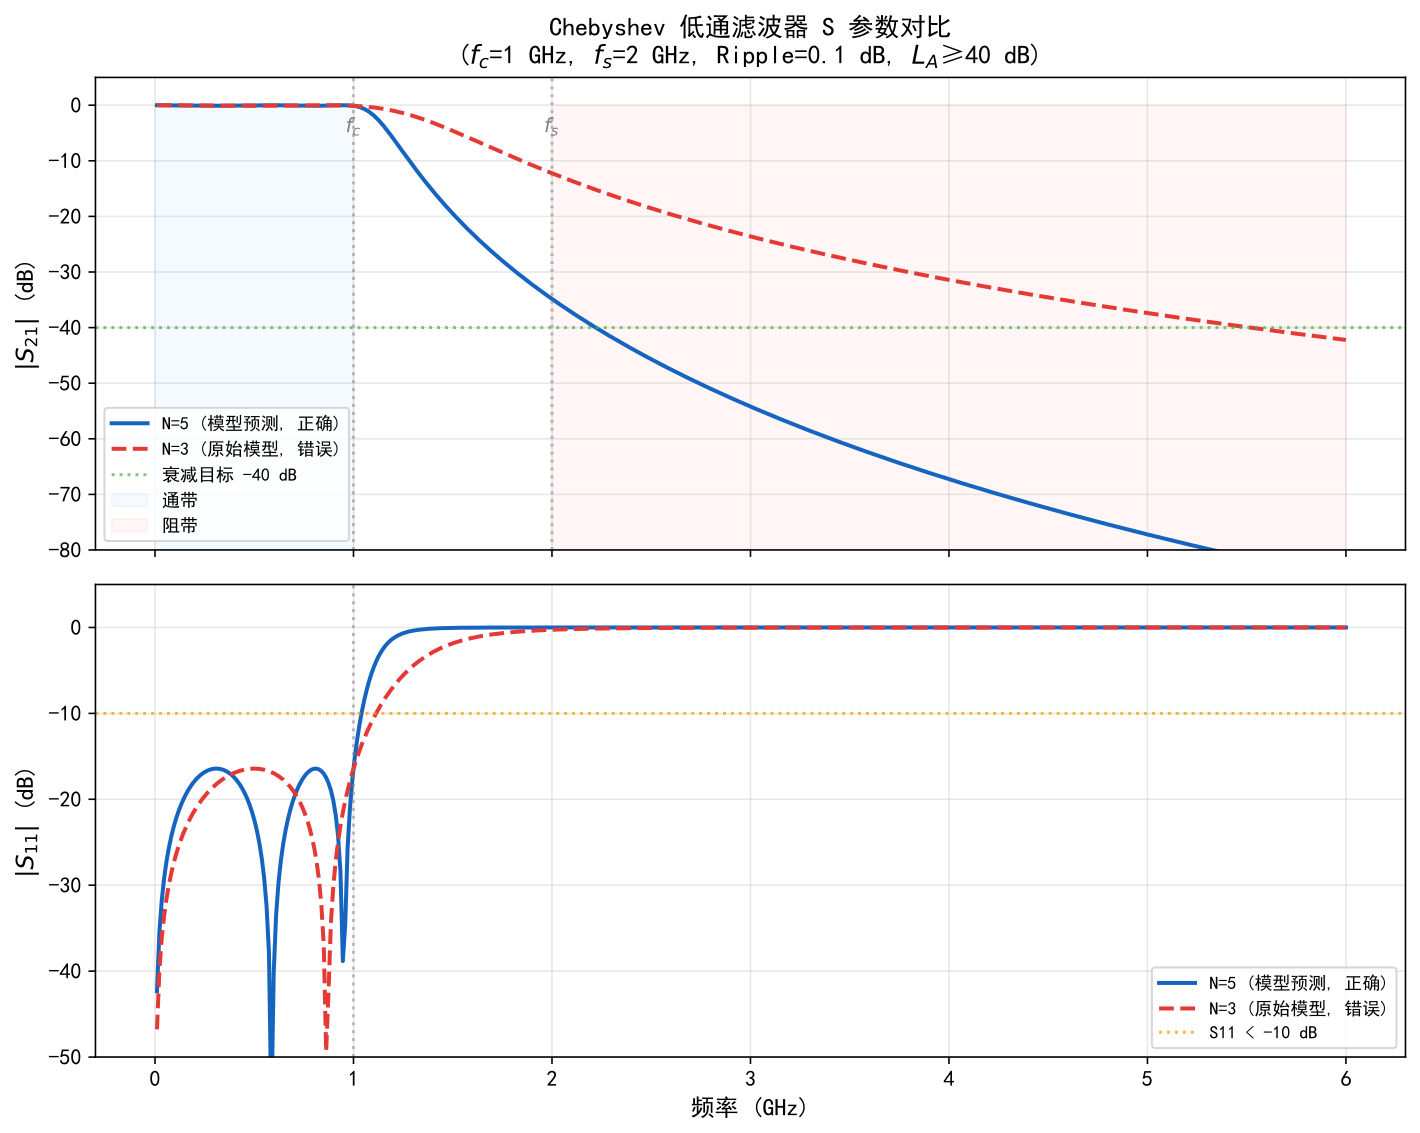
\includegraphics[width=\columnwidth]{figs/sparam_lpf_comparison.pdf}
\caption{S参数对比:正确阶数($N\!=\!5$,实线)与\ 错误($N\!=\!3$,虚线)的切比雪夫低通滤波器(LPF)。预测滤波器的阻带衰减未能达到$>$20\,dB。}
\label{fig:sparam}
\end{figure}

\subsection{Closed-Loop Agent Validation}

我们对切比雪夫低通滤波器($f_c\!=\!1$\,GHz,纹波$\!=\!0.5$\,dB,$R_0\!=\!50$\,$\Omega$)进行了验证。智能体在\textbf{2~次迭代}中收敛:迭代~1生成$S_{11}\!=\!-9.6$\,dB($>-10$\,dB阈值,FAIL);模型诊断出``通带匹配不足''并自主将纹波从0.5降低至0.25\,dB,使迭代~2达到$S_{11}\!=\!-12.4$\,dB(PASS)。这证明了基于物理的因果推理——而非盲目搜索。

\subsection{Comparison with Related Work}

Table~ 将我们的工作与现有方法进行对比。射频滤波器大语言模型(RF-FilterLLM)是唯一实现微调、多频段、本地可部署的LLM,其设计包含基于物理的闭环结构,并具备定量阶数精度基准测试能力。

\begin{table}[t]
\centering
\caption{Comparison with Existing Methods}
\label{tab:compare}
\setlength{\tabcolsep}{3pt}
\begin{tabular}{lcccccc}
\toprule
Method & FT? & Bands & Acc$_N$ & Local & Loop & Cost \\
\midrule
WiseEDA~\cite{wiseeda} & \xmark & LPF & N/R & \xmark & PSO & API \\
ChipChat~\cite{chipchat} & \xmark & N/A & N/A & \xmark & \xmark & API \\
ChipGPT~\cite{chipgpt} & \xmark & N/A & N/A & \xmark & \xmark & API \\
Baseline & \xmark & 3 & 19.5 & \cmark & \xmark & -- \\
\textbf{Ours} & \cmark & \textbf{3} & \textbf{83.4} & \cmark & \textbf{Refl.} & \textbf{9.4h} \\
\bottomrule
\end{tabular}
\end{table}

%=====================================================================
\section{Conclusion}
%=====================================================================

我们提出了RF-FilterLLM,一个通过高效大语言模型(LLM)微调实现射频滤波器自动设计的框架。通过由PIR、BPP和灵敏度分析流程增强的25,168个样本RF-Filter-SFT数据集,以及课程排序的QLoRA微调(0.047\%参数,9.4\,h在1$\times$~RTX~4090上),我们将滤波器阶数预测从19.5\%提升至83.4\%,同时达到100\% JSON合规性。消融实验表明数据增强至关重要---简单微调\emph{降低}性能。灵敏度引导的反思智能体通过ADS实现了物理信息迭代优化,仅需2~次迭代即可收敛。未来工作包括带通滤波器(BPF)特异性过采样、椭圆滤波器支持和跨模型迁移。

\begin{thebibliography}{00}
\bibitem{wiseeda} Y.~Zhang \emph{et al.}, ``WiseEDA: An LLM-assisted automated design framework for RF circuits,'' \emph{IEEE Trans. Microw. Theory Techn.}, 2024.
\bibitem{chipchat} J.~Blocklove \emph{et al.}, ``Chip-Chat: Challenges and opportunities in conversational hardware design,'' in \emph{Proc. ACM/IEEE DAC}, 2023.
\bibitem{chipgpt} K.~Chang \emph{et al.}, ``ChipGPT: How far are we from natural language hardware design,'' \emph{arXiv:2305.14019}, 2023.
\bibitem{lora} E.~J.~Hu \emph{et al.}, ``LoRA: Low-rank adaptation of large language models,'' in \emph{Proc. ICLR}, 2022.
\bibitem{qlora} T.~Dettmers \emph{et al.}, ``QLoRA: Efficient finetuning of quantized language models,'' in \emph{Proc. NeurIPS}, 2023.
\bibitem{matthaei} G.~L.~Matthaei, L.~Young, and E.~M.~T.~Jones, \emph{Microwave Filters, Impedance-Matching Networks, and Coupling Structures}.\hskip 1em plus 0.5em minus 0.4em Norwood, MA: Artech House, 1980.
\bibitem{curriculum} Y.~Bengio \emph{et al.}, ``Curriculum learning,'' in \emph{Proc. ICML}, 2009.
\bibitem{reflexion} N.~Shinn \emph{et al.}, ``Reflexion: Language agents with verbal reinforcement learning,'' in \emph{Proc. NeurIPS}, 2023.
\bibitem{llamafactory} Y.~Zheng \emph{et al.}, ``LlamaFactory: Unified efficient fine-tuning of 100+ language models,'' in \emph{Proc. ACL System Demonstrations}, 2024.
\end{thebibliography}

\end{document}